\documentclass{article}

\usepackage[utf8]{inputenc}     % pdfLaTeX
\usepackage[T1]{fontenc}
\usepackage[magyar]{babel}

\usepackage{amsthm}
\usepackage{amsmath}
\usepackage{amsfonts}

\usepackage{tikz}
\usetikzlibrary{arrows.meta, positioning}
\usepackage{graphicx}

\newtheorem{definition}{Definíció}
\newtheorem{corollary}{Folyomány}
\newtheorem{lemma}{Lemma}
\newtheorem{theorem}{Tétel}
\newtheorem{remark}{Megjegyzés}
\newtheorem{example}{Példa}

\title{Gráfelmélet}
\author{Rovenszky Robin}
\date{Legutóbb frissítve: 2026. Április 13.}

\begin{document}

\maketitle
\tableofcontents
\newpage

\section{Bevezető}

Háromféleképpen fogunk ábrázolni adatokat.

\begin{enumerate}
\item Felsorolásos forma: \\ \\
\begin{center}
    $\begin{matrix}
    A & B & C & D & E\\
    AB & AC & BC & DE & EE
    \end{matrix}$
\end{center}

\item Gráfábrázolás: \\ \\
\begin{center}
    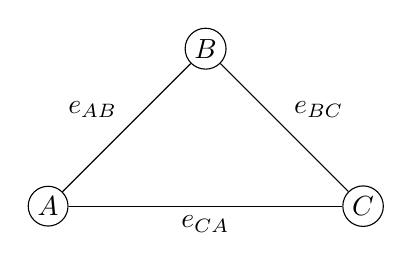
\begin{tikzpicture}[
        vertex/.style={circle, draw, inner sep=1.5pt},
        >=Stealth]
    
    \node[vertex] (A) at (0,0) {$A$};
    \node[vertex] (C) at (4,0) {$C$};
    \node[vertex] (B) at (2,2) {$B$};
    \draw[-] (A) -- node[above left] {$e_{AB}$} (B);
    \draw[-] (B) -- node[above  right] {$e_{BC}$} (C);
    \draw[-] (A) -- node[below] {$e_{CA}$} (C);
    
    \end{tikzpicture}
\end{center}

\item Mátrixos forma: \\ \\
\begin{center}
    $\begin{matrix}
     & A & B & C & D & E \\
     A & 0 & 1 & 1 & 0 & 0\\
     B & 1 & 0 & 1 & 0 & 0\\
     C & 1 & 1 & 0 & 0 & 0\\
     D & 0 & 0 & 0 & 0 & 1\\
     E & 0 & 0 & 0 & 1 & 1
    \end{matrix}$
\end{center}
\end{enumerate}

\section{Definíciók}
\begin{definition}[Irányítatlan gráf]
    Csúcsokból és élekből áll. Egy él két, nem feltétlenül különböző csúcsot köt össze.
\end{definition}


\begin{definition}[Hurokél]
    Olyan él, amely egy csúcsot önmagához köt.
\end{definition}

\begin{center}
    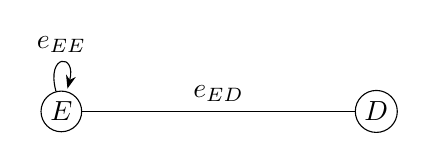
\begin{tikzpicture}[
            vertex/.style={circle, draw, inner sep=1.5pt},
            >=Stealth]
            
        \node[vertex] (E) at (0,-2) {$E$};
        \node[vertex] (D) at (4,-2) {$D$};
        \draw[-] (E) -- node[above] {$e_{ED}$} (D);
        \draw[-] (E) edge[loop above] node {$e_{EE}$} ();
        
    \end{tikzpicture}
\end{center}


\begin{definition}[Többszörös él]
    Egy él akkor többszörös él, ha létezik legalább egy másik él amely ugyan azt a két csúcsot köti össze.
\end{definition}

\begin{center}
    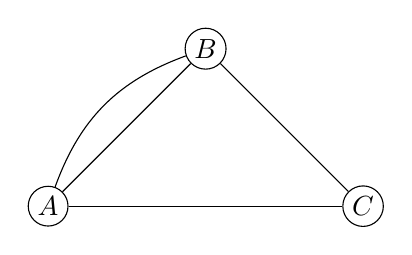
\begin{tikzpicture}[
        vertex/.style={circle, draw, inner sep=1.5pt},
        >=Stealth
    ]
    
    \node[vertex] (A) at (0,0) {$A$};
    \node[vertex] (C) at (4,0) {$C$};
    \node[vertex] (B) at (2,2) {$B$};
    
    \draw[-] (A) -- (B);
    \draw[-] (B) -- (C);
    \draw[-] (A) -- (C);
    
    \draw[-, bend left=25] (A) to (B);
    
    \end{tikzpicture}
\end{center}


\begin{definition}[Egyszerű gráf]
    Olyan gráf, melynek nincs hurokélje és többszörös élje.
\end{definition}

\begin{definition}[Összefüggő gráf]
    Olyan gráf, melynek bármely pontjából bármely másik pontjába vezet út.
\end{definition}

\begin{definition}[Komponens]
    Olyan részgráf, amely összefüggő és a csúcsok számára nézve maximális.
\end{definition}

\begin{definition}[Fokszám]
    Adott csúcs fokszáma megadja az adott csúcsot elhagyó élek számát. Adott gráf fokszáma megadja az gráfban lévő csúcsok fokszámainak összegét.
\end{definition}

\begin{definition}[Üres gráf]
    Olyan gráf, melynek fokszáma 0.
\end{definition}

\begin{definition}[Teljes gráf]
    Olyan gráf, mely a fokszámára való tekintettel maximális, tehát minden csúcs minden csúccsal össze van kötve.
\end{definition}

\begin{definition}[Út]
    Egymáshoz kapcsolódó élek egymásutánja. Se él, se csúcs nem ismétlődik benne.
\end{definition}

\begin{definition}[Vonal]
    Olyan út, amelyben a csúcsok ismétlődhetnek.
\end{definition}

\begin{definition}[Séta]
    Olyan vonal, amely megengedi az élek ismétlődését.
\end{definition}

\begin{definition}[Kör]
    Olyan út, melynek kezdő és végpontja megegyezik.
\end{definition}

\begin{definition}[Hamilton-út]
    A gráf összes csúcsát tartalmazó út.
\end{definition}

\begin{definition}[Hamilton-kör]
    A gráf összes csúcsát tartalmazó kör.
\end{definition}

\begin{definition}[Euler-vonal]
    A gráf összes élét tartalmazó vonal.
\end{definition}

\begin{definition}[Euler-kör]
    A gráf összes élét tartalmazó kör.
\end{definition}

\begin{lemma}
    Egy összefüggő gráf komponenseinek száma 1.
\end{lemma}
\begin{proof}
    Tegyük fel, hogy adott gráf $G$ összefüggő. Egy komponens definíció szerint létezik. Válasszunk ki kettő vagy több részgráfot. Válasszunk ki annyi csúcsot, amennyi részgráfot. Mivel a gráf összefüggő, a pontok között léteznek utak, tehát a részgráfok a csúcsok számára nézve nem maximálisak, tehát nem komponensek.
\end{proof} % TODO: Better proof

\section{Fák}
\begin{definition}[Fa]
    Egyszerű, összefüggő, körmentes gráf.
\end{definition}

\end{document}